\subsection{Interface}
    \subsubsection{config.php}
        Creates an array that will give the main location to the API and declares the directory that the sessions will be  stored in.

    \subsubsection{header.php}
        \begin{itemize}
            \item includes config.php
            \item Error reporting
            \begin{itemize}
                \item On the occurrence of an error, error messages are removed and not displayed
            \end{itemize}
            \item Meta data
            \begin{itemize}
                \item This declares the meta information for the site such the author and the site description
            \end{itemize}
            \item title declaration
            \begin{itemize}
                \item Echos the title of the page that is declared on each of the individual pages
            \end{itemize}
            \item CSS links
            \begin{itemize}
                \item Links to all the CSS files 
            \end{itemize}
            \item Login functions
            \begin{itemize}
                \item If the password session does not exist, then the authentication form is displayed. If the authentication session exists, then a logout is displayed 
            \end{itemize}
            \item Navigation
            \begin{itemize}
                \item Creates a constant header throughout the website.
            \end{itemize}
            \item Messages
            \begin{itemize}
                \item When the authentication or logout method is called, it will either display a success, error, or logout message 
            \end{itemize}
        \end{itemize}

    \subsubsection{footer.php}
        The footer will be ending specific div tags from the page and the header.

    \subsubsection{Authenticate.php}
        \begin{itemize}
            \item includes config.php 
            \item Check authentication form is submitted
            \begin{itemize}
                \item The script checks if a password has been submitted and attaches the string to a session.
            \end{itemize}
            \item Authentication CURL POST request
            \begin{itemize}
                \item First gets the password session variable and sets the variables.Then uses a variable to connect to the API method through the config file. It will then set the url, the number of POST variables and the data being sent. The server will then reply with a response message stating if the password is correct, it is true, where a message will be generated. If it is false, then a login error message will be sent to the previous page and the session will be destroyed.
            \end{itemize}
        \end{itemize}

    \subsubsection{index.php}
        \begin{itemize}
            \item Title variable
            \begin{itemize}
                \item The title is attached to a variable that is then called within the header
            \end{itemize}
            \item Include header.php
            \item Simple search form
            \begin{itemize}
                \item This form will search for a species name that matches any of the data that is inputted inside of the form. The user will be taken to the plant species page where the search results will be displayed.
            \end{itemize}
            \item Include footer.php
        \end{itemize}
    
        
    \subsubsection{reserves.php}
        \begin{itemize}
            \item Title variable
            \begin{itemize}
                \item The title is attached to a variable that is then called within the header
            \end{itemize}
            \item include header.php
            \item include reserves\_curl.php
            \begin{itemize}
                \item includes the script that gets all the reserves from the server.
            \end{itemize}
            \item Declaration of reserve variables
            \begin{itemize}
                \item A for each loop will go through all of the reserve objects and attach them to a new variable. The new variable will then attach the data for a variable that is easily recognizable and usable.
            \end{itemize}
            \item Admin functions
            \begin{itemize}
                \item If the password session exists, then the user will be able to have more options for each reserves. If they are authenticated, then the user can delete and edit the reserve. If they are not, they do not get the option to do this.
            \end{itemize}
        \end{itemize}
    

    \subsubsection{reserves\_curl.php}
        \begin{itemize}
            \item includes config.php 
            \begin{itemize}
                \item includes the config file that holds the information to access the web API and the session directory
                \item First it uses a variable to connect to the API method through the config file. It will then set the url, the number of POST variables and the data being sent, which will get the order and method function, and the methods declared for that function. THe data is then sent, and then received back from the server, which will contain the JSON object, which will then be decoded and assigned to a variable for practical use. The request is then sent, and the connection is closed
            \end{itemize}
        \end{itemize}


    \subsubsection{add\_reserve.php}
        \begin{itemize}
            \item Title variable
            \begin{itemize}
                \item The title is attached to a variable that is then called within the header
            \end{itemize}
            \item Include header.php
            \item Add reserve form
            \begin{itemize}
                \item This form will be used to input the data that will be sent to the web API via a POST request.
            \end{itemize}
            \item addReserve POST request 
            \begin{itemize}
                \item First it uses a variable to connect to the api method through the config file. The page will have a form inside of it that will POST data, that will then be caught within an array. This array will then be encoded into json and this is assigned to a variable. The script will then set the url, the number that is being posted which will be the single record and then get a response. The POST request will then be closed.
            \end{itemize}
            \item include footer.php
        \end{itemize}

    \subsubsection{edit\_reserve.php}
        \begin{itemize}
            \item Title declaration
            \begin{itemize}
                \item The title is attached to a variable that is then called within the header
            \end{itemize}
            \item include header.php
            \item Authentication session confirmation
            \begin{itemize}
                \item If there is no session, then the user will be redirected to the reserve page.
            \end{itemize}
            \item include get\_reserve.php
            \item Edit reserve form
            \begin{itemize}
                \item This form will be the same as the add reserve function, however, the values will be already there from an existing reserve, that will get the reserveID that has been posted. Th reserveID will be in a hidden input type so the ID will be recognized for the editing of the reserve. This form will be used to input the data that will be sent to the web API via a POST request.
            \end{itemize}
            \item editReserve POST request
            \begin{itemize}
                \item First the POST request checks that the location name has been submitted, and then it uses a variable to connect to the api method through the config file. The page will have a form inside of it that will POST data, that will then be caught within an array. This array will then be encoded into JSON and this is assigned to a variable. The script will then set the url, the number that is being posted which will be the single record and then get a response. The POST request will then be closed. Once the script has finished, the user will be redirected to the reserves page.
            \end{itemize}
            \item include footer.php
        \end{itemize}

    \subsubsection{get\_reserve.php}
        \begin{itemize}
            \item include config.php
            \item getReserve POST request
            \begin{itemize}
                \item First it uses a variable to connect to the API method through the config file. The script will be using a GET method to get the resID that the user is editing. The script will then set the url, the number that is being posted which will be the single record and then get a response. Once the response is available, it will be decoded from JSON to an array to an object. The POST request is then closed.
            \end{itemize}
        \end{itemize}

    \subsubsection{plant\_specimens.php}
        \begin{itemize}
            \item Title variable
            \begin{itemize}
                \item The title is attached to a variable that is then called within the header
            \end{itemize}
            \item include header.php
            \item include specimens\_curl.php
            \item include filter.php
            \item Search form
            \begin{itemize}
                \item This form allows the user to select a searching filter (species, user name, or location name), and lets them input a textual value for the selected filter.
            \end{itemize}
            \item Sort form
            \begin{itemize}
                \item This form allows the user to sort the list of specimens by a selected field and pick sorting order. It also includes pagination controls (next page/previous page).
            \end{itemize}
            \item Results table
            \begin{itemize}
                \item The results table is where the results of the current search/sort are being displayed. It is accessed by the client-side script and updated with new rows whenever
                new search results are ready.
            \end{itemize}
            \item Client-side scripts
            \begin{itemize}
                \item Showing the user search results is performed asynchronously, by calling the website back-end using a POST request. The back-end in turn goes to the Web API, and
                performs a search request. The Web API returns a JSON-formatted array of specimen results, which gets send back to the client-side for processing and visualisation.
                
                \item The script is able to react instantaneously to user input by placing event handlers on controls in both the sort and search forms, triggering a new request whenever
                a change in values is detected. The search value text field inside the search form makes an exception -- instead reacting instantaneously to changes in the text value,
                the script polls the content of the text field every second, and then decides whether to perform a new request to the back-end, thus avoiding an unnecessarily large amount
                of requests being sent.
            \end{itemize}
        \end{itemize}
    

    \subsubsection{filter.php}
        \begin{itemize}
            \item This file starts with a new div tag that will contain the form that will allow the user to filter and sort the results. Once the this div section ends, the pagination will be there, where they will just be buttons.
        \end{itemize}

    \subsubsection{add\_specimens.php}
        \begin{itemize}
            \item Title variable
            \begin{itemize}
                \item The title is attached to a variable that is then called within the header
            \end{itemize}
            \item include header.php 
            \item include reserve\_list.php
            \item add specimen form
            \begin{itemize}
                \item This form will allow the user to input the data concerning the specimen. This will then be posted to be available to be used in the POST request.
            \end{itemize}
            \item include footer.php
            \item add\_resource POST request
            \begin{itemize}
                \item First it uses a variable to connect to the API method through the config file. It will then set out the options for the CURL POST request. However, if there is no image uploaded, then it will be assigned -1, which will make it that it does not exist. There will be another script basically the same for the other image that will be uploaded.
            \end{itemize}
            \item Addrecord
            \begin{itemize}
                \item An array will be created for all of the fields that will be inputted in the form. Before the submit, they will be empty, and once the form is submitted, the form will POST the data into the array. There will be two arrays for this, the first will be specifically for the specimen and the second will be for the user details. The two arrays will be then encoded into json and sent to the API.
            \end{itemize}
        \end{itemize}
        
    \subsubsection{reserve\_list.php}
        \begin{itemize}
            \item This script will use a POST request that will get all of the reserves, and then put them into an array so they can only existing reserves can be selected.
        \end{itemize}

    \subsubsection{edit\_specimens.php}
        \begin{itemize}
            \item Title variable
            \begin{itemize}
                \item The title is attached to a variable that is then called within the header
            \end{itemize}
            \item include header.php 
            \item include record\_curl.php
            \item Edit specimen form
            \begin{itemize}
                \item This form will allow the user to input the data concerning the specimen. The existing data for the specimens will already be inputted. There will be a hidden field for the ID so that the specimen that is meant to be edited is updated. This will then be posted to be available to be used in the POST request.
            \end{itemize}
            \item include footer.php
            \item editResource POST request
            \begin{itemize}
                \item First it uses a variable to connect to the API method through the config file. It will then set out the options for the CURL POST request. However, if there is no image uploaded, then it will be assigned -1, which will make it that it does not exist. There will be another script basically the same for the other image that will be uploaded.
            \end{itemize}
            \item editRecord POST request
            \begin{itemize}
                \item An array will be created for all of the fields that will be inputted in the form. Before the submit, they will be empty, and once the form is submitted, the form will POST the data into the array. There will be two arrays for this, the first will be specifically for the specimen and the second will be for the user details. The two arrays will be then encoded into json and sent to the API. 
            \end{itemize}
        \end{itemize}


    \subsubsection{specimen.php}
        \begin{itemize}
            \item Title variable
            \begin{itemize}
                \item The title is attached to a variable that is then called within the header
            \end{itemize}
            \item include record\_curl.php
            \item include header.php
            \item include img\_curl.php
            \item Specimen checker
            \begin{itemize}
                \item If a user were to go the specimen page with no id submitted, then they user will be redirected to plant\_specimens page.
            \end{itemize}
            \item LatLong Map
            \begin{itemize}
                \item Because the map is in a separate page, the lat and the long will be included into a session, where it can then be transferred when the map pop up is shown.
            \end{itemize}
            \item Specimen table
            \begin{itemize}
                \item The specimen details will be stored inside of a html table, where they will be presented in a horizontal alignment. Each field data will be received by the record\_curl post request include, where it will then be available through through the decoded object. The images will be the same, but with two POST requests for each of the images.
            \end{itemize}
            \item Default Picture
            \begin{itemize}
                \item On the occurrence that a specimen does not have an image attached to it, there will be a Jquery script that will give a default image in its place. If there is an error with getting the image, then it will replace the broken image link with the default.
            \end{itemize}
            \item Session Authentication options
            \begin{itemize}
                \item If the password session exists, then the user will be able to have two more options for the specimen. They can either edit the specimen or they can delete the specimen. However, if the session does not exist, then the buttons will not exist.
            \end{itemize}
            \item include footer.php
        \end{itemize}


    \subsubsection{remove\_curl.php}
        \begin{itemize}
            \item include config.php
            \item removeSpecimen POST Request
            \begin{itemize}
                \item First it uses a variable to connect to the API method through the config file. Then an array will be created that will be storing the id by use of the GET method, and checking if there is a  password session.
                \item The script will then set the url, the number that is being posted which will be the single record and then get a response. If the response is 200 then the specimen is deleted. The POST request is then closed.
            \end{itemize}
        \end{itemize}

    \subsubsection{about.php}
        \begin{itemize}
            \item Title variable
            \begin{itemize}
                \item The title is attached to a variable that is then called within the header
            \end{itemize}
            \item include header.php
            \item include footer.php
        \end{itemize}

    \subsubsection{img\_curl.php}
        \begin{itemize}
            \item include config.php
            \item getResource POST request
            \begin{itemize}
                \item There will be two separate POST requests that will do the exact same thing, however, they will be different because there are two pictures that will be recieved. First it uses a variable to connect to the API method through the config file. Then an array will be created that will be storing the resourceID that is declared through the record\_curl.php page. The script will then set the url, the number that is being posted which will be the single record and then get a response. If the response is 200 then the specimen is deleted. The POST request is then closed.
            \end{itemize}
        \end{itemize}
        
    \subsubsection{logout.php}
        \begin{itemize}
            \item include config.php
            \item Logout function
            \begin{itemize}
                \item As the user is only allowed to have administrative permissions if the password session exists, the user will want to logout. This page basically just destroys the session, which it then creates a message that notifies the user that the user has been logged out.
            \end{itemize}
        \end{itemize}

    \subsubsection{map.php}
        \begin{itemize}
            \item include config.php
            \item Google Map API
            \begin{itemize}
                \item The Google map will be in its own separate page because we will be using an iframe to view the map through, that will be viewable on the specimens page. The script first gets the API from Google, then creates the location where it wants to centre onto, which the information will be stored inside of a session. The function is initialised with specific options such as the zoom and the type of map. The map is then set. In the body, the map is then created.
            \end{itemize}
        \end{itemize}

    \subsubsection{res\_remove.php}
        \begin{itemize}
            \item include config.php
            \item removeRemove POST Request
            \begin{itemize}
                \item First it uses a variable to connect to the API method through the config file. Then an array will be created that will be storing the id by use of the GET method, and checking if there is a  password session.
                \item The script will then set the url, the number that is being posted which will be the single record and then get a response. If the response is 200 then the specimen is deleted. The POST request is then closed.
            \end{itemize}
        \end{itemize}

\subsection{Detailed design}

    \subsubsection{index.php}
        This is the front page of the website to the user, it contains a description of the purpose of the site.

        
    \subsubsection{about.php}
        This page contains a short description about the app as well as the team.

        
    \subsubsection{reserves.php}
        This page contains a script to display the data from the json object for the reserves. It includes scripts to retrieve the json oject as well as to delete the json ojects.

        
    \subsubsection{add\_reserve.php}
        The page gives the user the ability to input data for a new reserve in to a html form. This page also contains a script to collect the data into a json object and a curl method to send the json object to the server.

        
    \subsubsection{edit\_reserve.php}
        Edit reserve returns the contents of a json object for reserve to a html form allowing the user to edit its details. A script to encode the reserve to a json object is also included in the page as well as a curl methodto send the json object to the server.

        
    \subsubsection{specimen.php}
        Specimen has a script to return the data from the json object to a table to display as a friendly interface to the user. There is scripts for navigation within the record, these create links to the next and previous specimens within the record. There is a script within the page which produces a pop-up map (using google maps) displaying the location of where this specimen was found. This page also contains scripts to include the site and specimen images.

        
    \subsubsection{add\_specimen.php}
        This page contains a html form to collect data from the user about a new specimen to be added. The page also contains a script to make the data into a new json object as well as a curl method to send the data to the server. There is a script to upload images which are then sent to a private folder via a curl method.

        
    \subsubsection{edit\_specimen.php}
        Edit specimen contains a script to retrieve the data from the specimen json object and places it in to a html form for the user to edit. There is also scripts to encode the edited data to a json object and to submit the object to the server via a curl method.

        
    \subsubsection{plant\_specimens.php}
        Plant specimens contains a script which allows the user to search the database to find a specific species. This page also contains 


    \subsubsection{config.php}
        The config.php file will be used to establish the connection to the mysql database using the servers API at the start of a new session.
        \begin{verbatim}
            $CONFIG=array
            api="file location"
            session="where the session is stored"
        \end{verbatim}
        The config.php will need to be be included in all php scripts.


    \subsubsection{authenticate.php}
        The authenticate.php script will be used to authenticate an admin user on the site. Who through entering a correct password will have access to certain features of the site that regular users will not have. Such as deletion of reserves and specimens. The authentication will be checked to the servers API. If a correct password is entered then the user will see a message confirming it. If an incorrect password is used then a different message will be see saying that a wrong password has been used.


    \subsubsection{delete\_curl.php}
        This script is used to delete specific specimens from the servers database. This feature will only become available once a user has entered a correct password to show that they are an admin user. PHP CURL is used so that the website can communicate with the server.


    \subsubsection{edit\_specimens.php}
        This script is similar to the delete script. It uses PHP CURL to communicate with the server. This function is also only available to admin users.


    \subsubsection{footer.php}
        This script will be included on every page. It will contain a small website logo in the centre of the footer. 


    \subsubsection{get\_reseve.php}
        This will be used to call all the data about the reserves stored on the server. PHP CURL will be used to communicate with the server and to decode the JSON that the API will be using so that it can be displayed on the reserves page.

    \subsubsection{header.php}
        The header will be responsible for creating a session and storing it for the users. The header script will be responsible for declaring the doctype and meta tags such as description, keywords, content type, CSS and font links, validation as well as JAVASCRIPT and the title. 

    \subsubsection{img\_curl.php}
        This is used to find get the specimen and scene photo from the database. PHP CURL is again used to communicate with th server.

    \subsubsection{logout.php}
        This script is used to logout an admin user who has entered a correct password to the site. It will end the session that is being used and display a message telling the user that they have been logout of the site.

    \subsubsection{map.php}
        The contains the JAVASCRPIT to be able to view the plants location within a Google maps pop up. It will use the latitude and longitude variables of each specimen to give an accurate location.

    \subsubsection{specimens\_curl.php}
        This will be used to access the information and each individual specimen. CURL is again used to access the server.

    \subsubsection{resdelete\_curl.php}
        This will work in a very similar way to the delete\_curl.php script but will be used for deleting whole reserves instead of just individual specimens. The user will need the be logged in for this function to work. 

    \subsubsection{reserves\_curl.php}
        Much like the record\_curl.php it will be used to get information form the server, but information about the reserves rather then the specimen details.

    \subsubsection{specimens\_search.php}
        This will be used to search for certain specimens within the specimen page on the website. Users will be able to search by Species Name, Location Name and The User Name of people using the site.

    \subsubsection{filter.php}
        This will also be used on the plants page on the website and will allow users to order by Species Name, Location, User Name, Date and Abundance and allow results to be show in ascending or descending order.

\begin{landscape}
    \begin{figure}
        \centering
        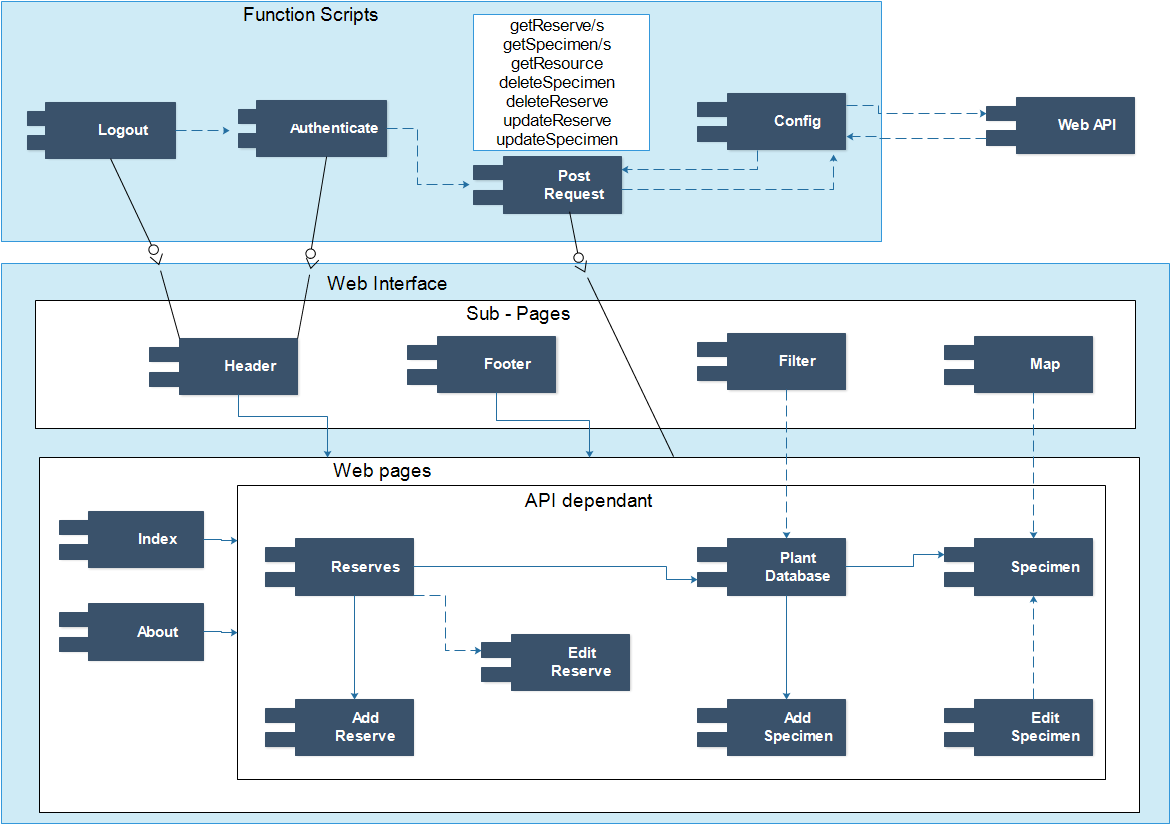
\includegraphics[scale=0.75]{web/webComponentDiagram.png}
        \caption{Web component Diagram}
        \label{fig:webComponentDiagram}
    \end{figure}
\end{landscape}


